\chapter{Part Part IV(c) - Instruction Level Parallelism}
In the last chapter, we've seen how pipelining can make it easier to parallelize indepent operations making it the overall process faster.

\subsection{Pipelining the Processor}
Pipelining in processors is a technique that splits the execution of an instruction into multiple stages, each handled in parallel by separate hardware units. By doing so, multiple instructions can be processed simultaneously, thereby increasing the overall throughput of the processor without increasing the clock frequency.

\begin{itemize}
    \item[-] \textbf{Fetch (F)}: Retrieve the instruction from memory (often from the instruction cache).
    \item[-] \textbf{Decode (D)}: Interpret the fetched instruction, identify operands, and configure the control signals for execution.
    \item[-] \textbf{Execute (E)}: Perform the required operations (e.g., arithmetic, logic, load, store).
\end{itemize}

\noindent In a basic pipeline with three stages (F, D, E), each stage takes one clock cycle. While one instruction is being executed, a second instruction can be decoded, and a third can be fetched at the same time. This overlapping of tasks leads to a substantial improvement in instruction throughput.

\subsubsection*{Example Pipeline Schedule}
Consider a schedule where three instructions (\(i\), \(i+1\), and \(i+2\)) enter the pipeline. Each instruction occupies a unique pipeline stage in any given clock cycle. Figure~\ref{fig:pipeline-schedule} illustrates how each instruction advances one stage every cycle:
\[
\begin{array}{c|cccccc}
\text{Time} & t & t+1 & t+2 & t+3 & t+4 & t+5 \\ \hline
i     & F & D & E & - & - & - \\
i+1   & - & F & D & E & - & - \\
i+2   & - & - & F & D & E & - \\
\end{array}
\]

\subsubsection*{Multi-Cycle Processor vs.\ Pipelined Processor}
A \emph{multi-cycle} processor might use multiple cycles to execute every instruction (e.g., separate cycles for Fetch, Decode, ALU, Memory Access, and Write Back), but only one instruction flows through the processor at a time. In contrast, a \emph{pipelined} processor allows the next instruction to begin its Fetch stage in parallel with the Decode stage of the previous instruction, greatly improving throughput.
\begin{center}
    \includegraphics[width=0.65\textwidth]{chapters/chapter4c/images/vs.png}
\end{center}
\subsubsection*{Key Observations for Pipelining}
\begin{enumerate}
    \item \textbf{Repetitive Activity}: Pipelining is effective only when the processor has a large number of instructions to execute.
    \item \textbf{Subactivities}: Each major task (Fetch, Decode, Execute, etc.) should be clearly separable into sub-stages to allow parallel operation.
    \item \textbf{Throughput Gain}: Once the pipeline is full, an instruction completes at the end of every cycle (in the ideal case), increasing throughput.
\end{enumerate}

\noindent Properly designing pipeline stages and handling hazards (such as data, control, and structural hazards) ensures that the pipeline delivers high performance without correctness issues.

\section{Hardware Reuse Across Processor Stages}

In processor design, the approach to hardware reuse varies significantly between multicycle and pipelined architectures. Understanding these differences is crucial for optimizing performance and resource utilization.

\subsection{Multicycle Processor Architecture}

A multicycle processor divides instruction execution into distinct \textbf{states}, allowing certain hardware components to be shared across these states. This sharing is feasible because the components are not required simultaneously, enabling efficient resource utilization.

\begin{itemize}
    \item \textbf{FETCH} State: Typically involves an \textit{adder} to increment the program counter (PC).
    \item \textbf{EXECUTE} State: Requires an \textit{Arithmetic Logic Unit} (ALU) to perform operations.
\end{itemize}

Since the \textit{adder} and the \textit{ALU} are not active concurrently, the ALU can be repurposed to increment the PC during the FETCH state. This reuse reduces the overall hardware complexity and cost.

\subsection{Pipelined Processor Architecture}

In contrast, a pipelined processor operates with multiple \textbf{stages} that are active simultaneously. Each stage performs a different part of the instruction execution process, necessitating dedicated hardware for each stage to avoid conflicts and ensure seamless parallelism.

\begin{itemize}
    \item All pipeline stages are \textit{active concurrently}, handling different instructions in each stage.
    \item Hardware components cannot be shared across stages since multiple instructions require access to the same resources simultaneously.
    \item Consequently, hardware must be \textit{replicated} where necessary to maintain pipeline efficiency and prevent bottlenecks.
\end{itemize}

The inability to share hardware across pipeline stages often leads to increased hardware requirements compared to multicycle processors. However, this replication is essential for achieving high instruction throughput and maximizing pipeline performance.
\newpage
\section{Two Main Challenges in Processor Design}

Designing efficient processors involves addressing several challenges. Two prominent issues are the \textbf{CISC vs. RISC} debate and \textbf{instruction independence}.

\subsection{CISC vs. RISC}
\begin{enumerate}
    \item \textbf{Pipeline Efficiency in CISC vs. RISC}
    \begin{itemize}
        \item[] \textbf{Question}: Can we construct a pipeline for a Complex Instruction Set Computer (CISC) that matches the efficiency of a pipeline designed for a Reduced Instruction Set Computer (RISC)?
        \item[] \textbf{Implications}:
        \begin{itemize}
            \item RISC architectures typically use simpler, fixed-length instructions, which are easier to pipeline efficiently.
            \item CISC architectures have more complex, variable-length instructions, potentially complicating pipeline design and reducing efficiency.
            \item The distinction influences processor complexity, performance, and power consumption.
        \end{itemize}
    \end{itemize}
    \item \textbf{Ensuring Correct Execution with Dependent Instructions}
    \begin{itemize}
        \item \textbf{Issue}: Instructions are often \textit{dependent} on the results of preceding instructions, violating the assumption of \textbf{instruction independence}.
        \item \textbf{Challenge}: Executing code correctly in the presence of such dependencies requires soxphisticated mechanisms to handle hazards, such as data forwarding or pipeline stalls.
    \end{itemize}
\end{enumerate}

Addressing instruction dependencies is critical for maintaining the integrity of program execution while striving for optimal pipeline performance. Techniques such as out-of-order execution and speculative execution are often employed to mitigate the impact of these dependencies.
\section{Multi-Cycle Execution Using an FSM}
In a multi-cycle processor design, each instruction's execution is broken down into multiple steps (states), and the processor transitions through these steps via an FSM.

\subsection{FSM vs.\ Pipeline}
While a pipeline has a fixed sequence of stages (fetch, decode, execute, memory, writeback) for any instruction, an FSM-based multi-cycle design can assign different numbers of steps to each instruction. The FSM transitions vary based on the instruction being executed.



\subsection{Adding Instructions in a Multi-Cycle Design}
When introducing new instructions (e.g., \texttt{lw} or \texttt{add}), the FSM must be extended to accommodate additional states. For example, \texttt{lw} requires computing the address and accessing memory, whereas \texttt{add} mainly requires using the ALU to perform arithmetic. \\
\begin{minipage}[t]{0.45\textwidth}
\textbf{Adding \texttt{add} instruction}\\
We can support the \texttt{add} operation without changing drastically the design, we just need to add it to the ALU.
\[
\text{Fetch} \; \rightarrow \; \text{Decode} \; \rightarrow \; \text{Execute} \; \rightarrow \; \text{Writeback}.
\]
\end{minipage}
\hfill
\vline
\hfill
\begin{minipage}[t]{0.45\textwidth}
\textbf{Adding \texttt{lw} instruction}\\
However, for supporting \texttt{lw} instruction, we need to introduce \textbf{memory} to our design, so we add new steps.
\[
\text{Fetch} \; \rightarrow \; \text{Decode} \; \rightarrow \; \text{Execute} \; \rightarrow \; \text{Memory} \; \rightarrow \; \text{Writeback}.
\]
\end{minipage}
\newpage

\subsection{Adding Instructions to a Pipelined Processor}
Let's look at how this looks like in a pipelined processor.\\
\textit{In this example, we suppose xor and add instructions are both well supported.}
\begin{center}
    \includegraphics[width=0.45\textwidth]{chapters/chapter4c/images/pipelined-proc.png}
\end{center}
Now, to support \texttt{lw} instruction, we need to add a memory steps, the problem here is that, in a pipelined processor, changes affect \textbf{all instructions}, meaning that now, an \texttt{add} instruction will also take 5 cycles to complete. Thus,
\begin{center}
    \includegraphics[width=0.45\textwidth]{chapters/chapter4c/images/pipelined-proc-lw.png}
\end{center}

\section{The Importance of the ISA (CISC vs.\ RISC)}
The Instruction Set Architecture (ISA) heavily influences how instructions map onto hardware. A single complex CISC instruction might perform multiple memory accesses and arithmetic operations. In contrast, a RISC instruction set typically emphasizes simplicity: each instruction performs a smaller, more uniform set of operations.

\subsection{A CISC Example}
Consider a hypothetical CISC instruction:
\[
\texttt{sub 8(t4), 0(t1), 0(t2)}
\]
This single instruction might:
\begin{enumerate}
    \item Read the value in memory at address \(\texttt{t2 + 0}\).
    \item Read another value in memory at address \(\texttt{t1 + 0}\).
    \item Subtract these two values.
    \item Finally, store the result in memory at address \(\texttt{t4 + 8}\).
\end{enumerate}
Such complexity can inflate pipeline latency for \emph{all} instructions if the pipeline must accommodate these multi-step operations within a single instruction.
\begin{center}
    \includegraphics[width=0.65\textwidth]{chapters/chapter4c/images/cisc.png}
\end{center}
\subsection{The RISC Alternative}

Instead of imposing a \textbf{huge penalty} to every simple instruction by making complex instructions possible, the RISC approach advocates for \textbf{only using similarly simple instructions} and building programs with these. \\
\begin{minipage}[htp]{0.45\textwidth}
    \begin{center}
        \begin{tabular}{c c c}
        \texttt{sub 8(t4), 0(t1), 0(t2)} & $\longrightarrow$ &
        \begin{minipage}{0.45\linewidth}
        \texttt{lw t3, 0(t1)} \\
        \texttt{lw t5, 0(t2)} \\
        \texttt{sub t3, t3, t5} \\
        \texttt{sw t3, 8(t4)}
        \end{minipage} \\
        \end{tabular}
        \end{center}
\end{minipage}
\hfill
\vline
\hfill
\begin{minipage}[htp]{0.45\textwidth}
    It turns out that while this is not the only approach, \textbf{it is a good one}, and we will follow it in this course. \\
    In practice, modern CPUs blend design philosophies, using pipelining and other advanced techniques while balancing the complexities of their ISAs. A clear understanding of these concepts---from how an FSM handles instruction steps to how a pipeline benefits from simpler instructions---is crucial to mastering processor design.
\end{minipage}

\subsection{MIPS Pipelining Example}

The MIPS architecture uses a 5-stage pipeline to execute instructions. These stages are: Fetch (F), Decode (D), Execute (E), Memory (M), and Writeback (W). Each instruction moves through these stages, enabling the overlapping of instruction execution, which improves performance by allowing multiple instructions to be processed simultaneously.
\begin{center}
    \includegraphics[width=0.45\textwidth]{chapters/chapter4c/images/pipelined-mips.png}
\end{center}
\begin{enumerate}
    \item \textbf{Fetch (F):} The instruction is fetched from the instruction memory.
    \item \textbf{Decode (D):} The instruction is decoded, and the required arguments are obtained from the register file.
    \item \textbf{Execute (E):} The required operation is performed in the Arithmetic Logic Unit (ALU), including address calculations for loads and stores.
    \item \textbf{Memory (M):} Access to data memory is performed if needed, particularly for load and store operations.
    \item \textbf{Writeback (W):} The result of the operation, whether from the ALU or memory, is written back to the register file.
\end{enumerate}

This pipelining model allows instructions to be executed in parallel, thus improving the throughput of the processor and allowing more efficient use of system resources.

\subsection{The Laundry Metaphor for Pipelining}
Pipelining in computer architecture can be explained using the laundry metaphor. Consider the tasks involved in doing laundry: washing, drying, folding, and putting away. Each of these steps represents a stage in the pipeline.
\begin{center}
    \includegraphics[width=0.65\textwidth]{chapters/chapter4c/images/laundry.png}
\end{center}
\begin{itemize}
    \item[-] \textbf{Sequential Execution:} In a sequential process, one load of laundry is completed through all stages before starting the next. This approach takes a long time because each load must wait for the previous one to finish.
    \item[-] \textbf{Parallel Execution:} If the subtasks are completely independent, multiple washing machines, dryers, and folders could be used simultaneously. However, this is often impractical due to resource limitations.
    \item[-] \textbf{Pipelined Execution:} In pipelining, multiple loads of laundry are processed simultaneously, with each load at a different stage. For example, while one load is being washed, another is dried, and a third is folded. This overlaps the tasks, significantly reducing total time.
\end{itemize}

\newpage
\subsection{Two Distinct Memory Interfaces in MIPS}
In a MIPS processor, two distinct memory interfaces are utilized to enhance performance by allowing concurrent operations: the \textbf{Instruction Cache} and the \textbf{Data Cache}. These interfaces are depicted in the following architecture:
\begin{center}
    \includegraphics[width=0.45\textwidth]{chapters/chapter4c/images/mips.png}
\end{center}
\begin{itemize}
    \item[-] The \textbf{Instruction Cache} is accessed during the \textbf{Fetch} (F) stage, retrieving instructions for execution.
    \item[-] The \textbf{Data Cache} is utilized during the \textbf{Memory} (M) stage, providing data required for processing.
\end{itemize}

The pipeline stages of the MIPS processor are as follows:
\begin{enumerate}
    \item \textbf{F (Fetch)}: Instructions are fetched from the Instruction Cache.
    \item \textbf{D (Decode)}: Instructions are decoded, and operands are prepared using the Register File (RF).
    \item \textbf{E (Execute)}: The instruction is executed.
    \item \textbf{M (Memory)}: Data is accessed from or written to the Data Cache.
    \item \textbf{W (Write-back)}: Results are written back to the register file.
\end{enumerate}

The separation of memory interfaces allows the Instruction and Data caches to operate simultaneously, enabling improved throughput and reduced bottlenecks in the pipeline. Additionally, the Register File (RF) facilitates data flow between the stages.

This dual-interface approach is critical for high-performance pipelined architectures, allowing overlapping of instruction fetch and memory access operations.

\subsection{Pipeline Registers and Their Contents}
In a pipelined processor, each stage contains a pipeline register that holds specific data required for the correct execution of instructions. The key contents of these registers are described as follows:
\begin{center}
    \includegraphics[width=0.65\textwidth]{chapters/chapter4c/images/pipe-registers.png}
\end{center}
\begin{itemize}
    \item[-] \textbf{Instruction Register (F stage):} Contains the instruction that has just been fetched from memory.
    \item[-] \textbf{Operand Registers (D stage):} Stores two 32-bit operands read from the register file (if applicable).
    \item[-] \textbf{ALU Control Bits (D to E stages):} Transferred to control the arithmetic logic unit (ALU) operations.
    \item[-] \textbf{Destination Register Identifier (E and M stages):} Holds the 5-bit number of the destination register, specifying where the result should be written, if required.
    \item[-] \textbf{ALU Result (M stage):} Stores the 32-bit result computed by the ALU for use in subsequent stages.
\end{itemize}

The flow of data across these registers ensures efficient execution of instructions while maintaining data dependencies and avoiding hazards. The proper design of pipeline registers is critical to the performance of a pipelined processor.

\subsection{Pipeline Initialization and Execution}
The Animation below illustrates the state of a pipelined processor during its execution.Initially, all pipeline stages contain \texttt{nop} (no operation) instructions, ensuring the pipeline is empty and ready to fetch the first instruction from memory.
\begin{center}
    \href{https://github.com/elazdi-al/comparch/raw/refs/heads/main/chapters/chapter4c/images/video.mp4}{\textbf{You can view an animation of the execution here.}}
\end{center}
\begin{itemize}
    \item \textbf{Pipeline Stages:}
    \begin{itemize}
        \item \texttt{F (Fetch):} Fetches the instruction from memory using the program counter (PC).
        \item \texttt{D (Decode):} Decodes the instruction and retrieves the required register values from the register file (RF).
        \item \texttt{E (Execute):} Executes arithmetic or logical operations as specified by the instruction.
        \item \texttt{M (Memory):} Accesses memory for load or store operations.
        \item \texttt{W (Write-back):} Writes the computed results back to the register file.
    \end{itemize}
    \item \textbf{Initial Program Counter:} Set to 1000, fetching the first instruction (\texttt{add \$r2, \$r0, \$r1}).
\end{itemize}

\begin{verbatim}
1000: add $r2, $r0, $r1
1004: sub $r5, $r3, $r4
1008: sw  $r6, 50($r7)
1012: lw  $r9, 20($r8)
1016: mul $r12, $r10, $r11
\end{verbatim}

\subsubsection{Pipeline Hazard: Data Dependency Error}
Pipeline hazards can disrupt the smooth execution of instructions in a pipelined processor. One common type of hazard is the \textbf{data dependency hazard}, which occurs when an instruction depends on the result of a previous instruction that has not yet completed its execution.
\begin{center}
    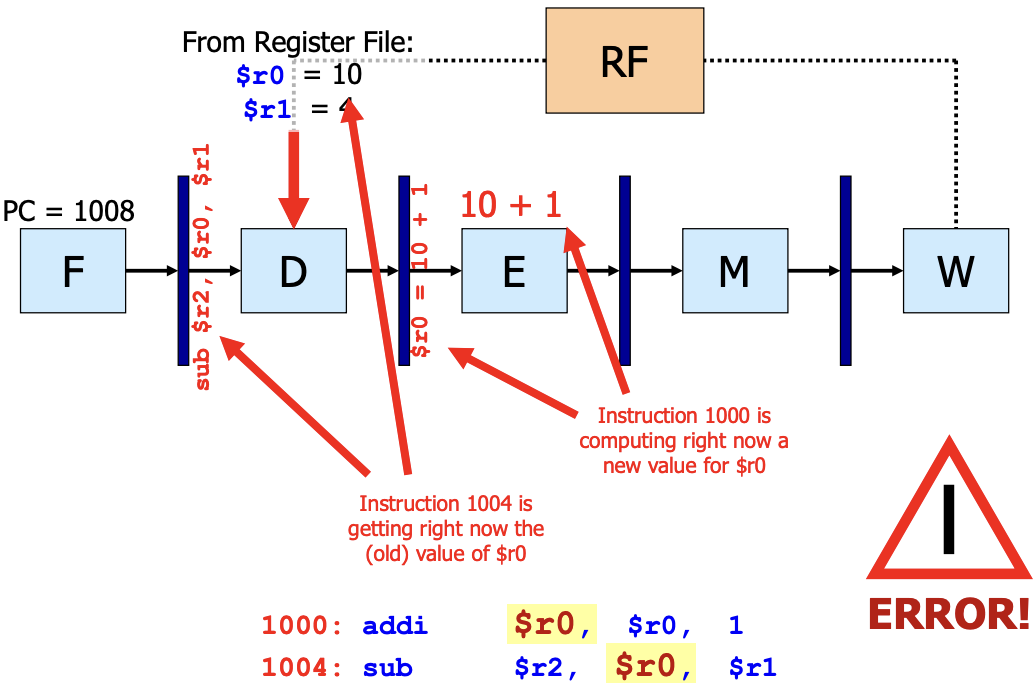
\includegraphics[width=0.55\textwidth]{chapters/chapter4c/images/problem.png}
\end{center}
Consider the following sequence of instructions executed in the previous example:
\begin{verbatim}
1000: addi $r0, $r0, 1
1004: sub $r2, $r0, $r1
\end{verbatim}

\begin{itemize}
    \item[-] At program counter (PC) 1000, the \texttt{addi} instruction modifies the value of register \texttt{\$r0} by incrementing it by 1.
    \item[-] At PC 1004, the \texttt{sub} instruction attempts to compute \texttt{\$r2} using the value of \texttt{\$r0}. However, it fetches the old value of \texttt{\$r0} from the register file because the result of the \texttt{addi} instruction is not yet available.
\end{itemize}

In this scenario, the \texttt{addi} instruction at PC 1000 is still in the \texttt{E} stage when the \texttt{sub} instruction at PC 1004 enters the \texttt{D} stage. Consequently, the \texttt{sub} instruction reads an outdated value of \texttt{\$r0}, leading to an incorrect result.

\section{Data Hazard Detection in Pipelined Processors}
Data hazards occur when instructions in a pipelined processor depend on the results of previous instructions that have not yet completed execution. To address this, the pipeline employs a hazard detection unit. The figure below illustrates the hazard detection mechanism for a sequence of instructions in a pipelined processor.

\begin{center}
    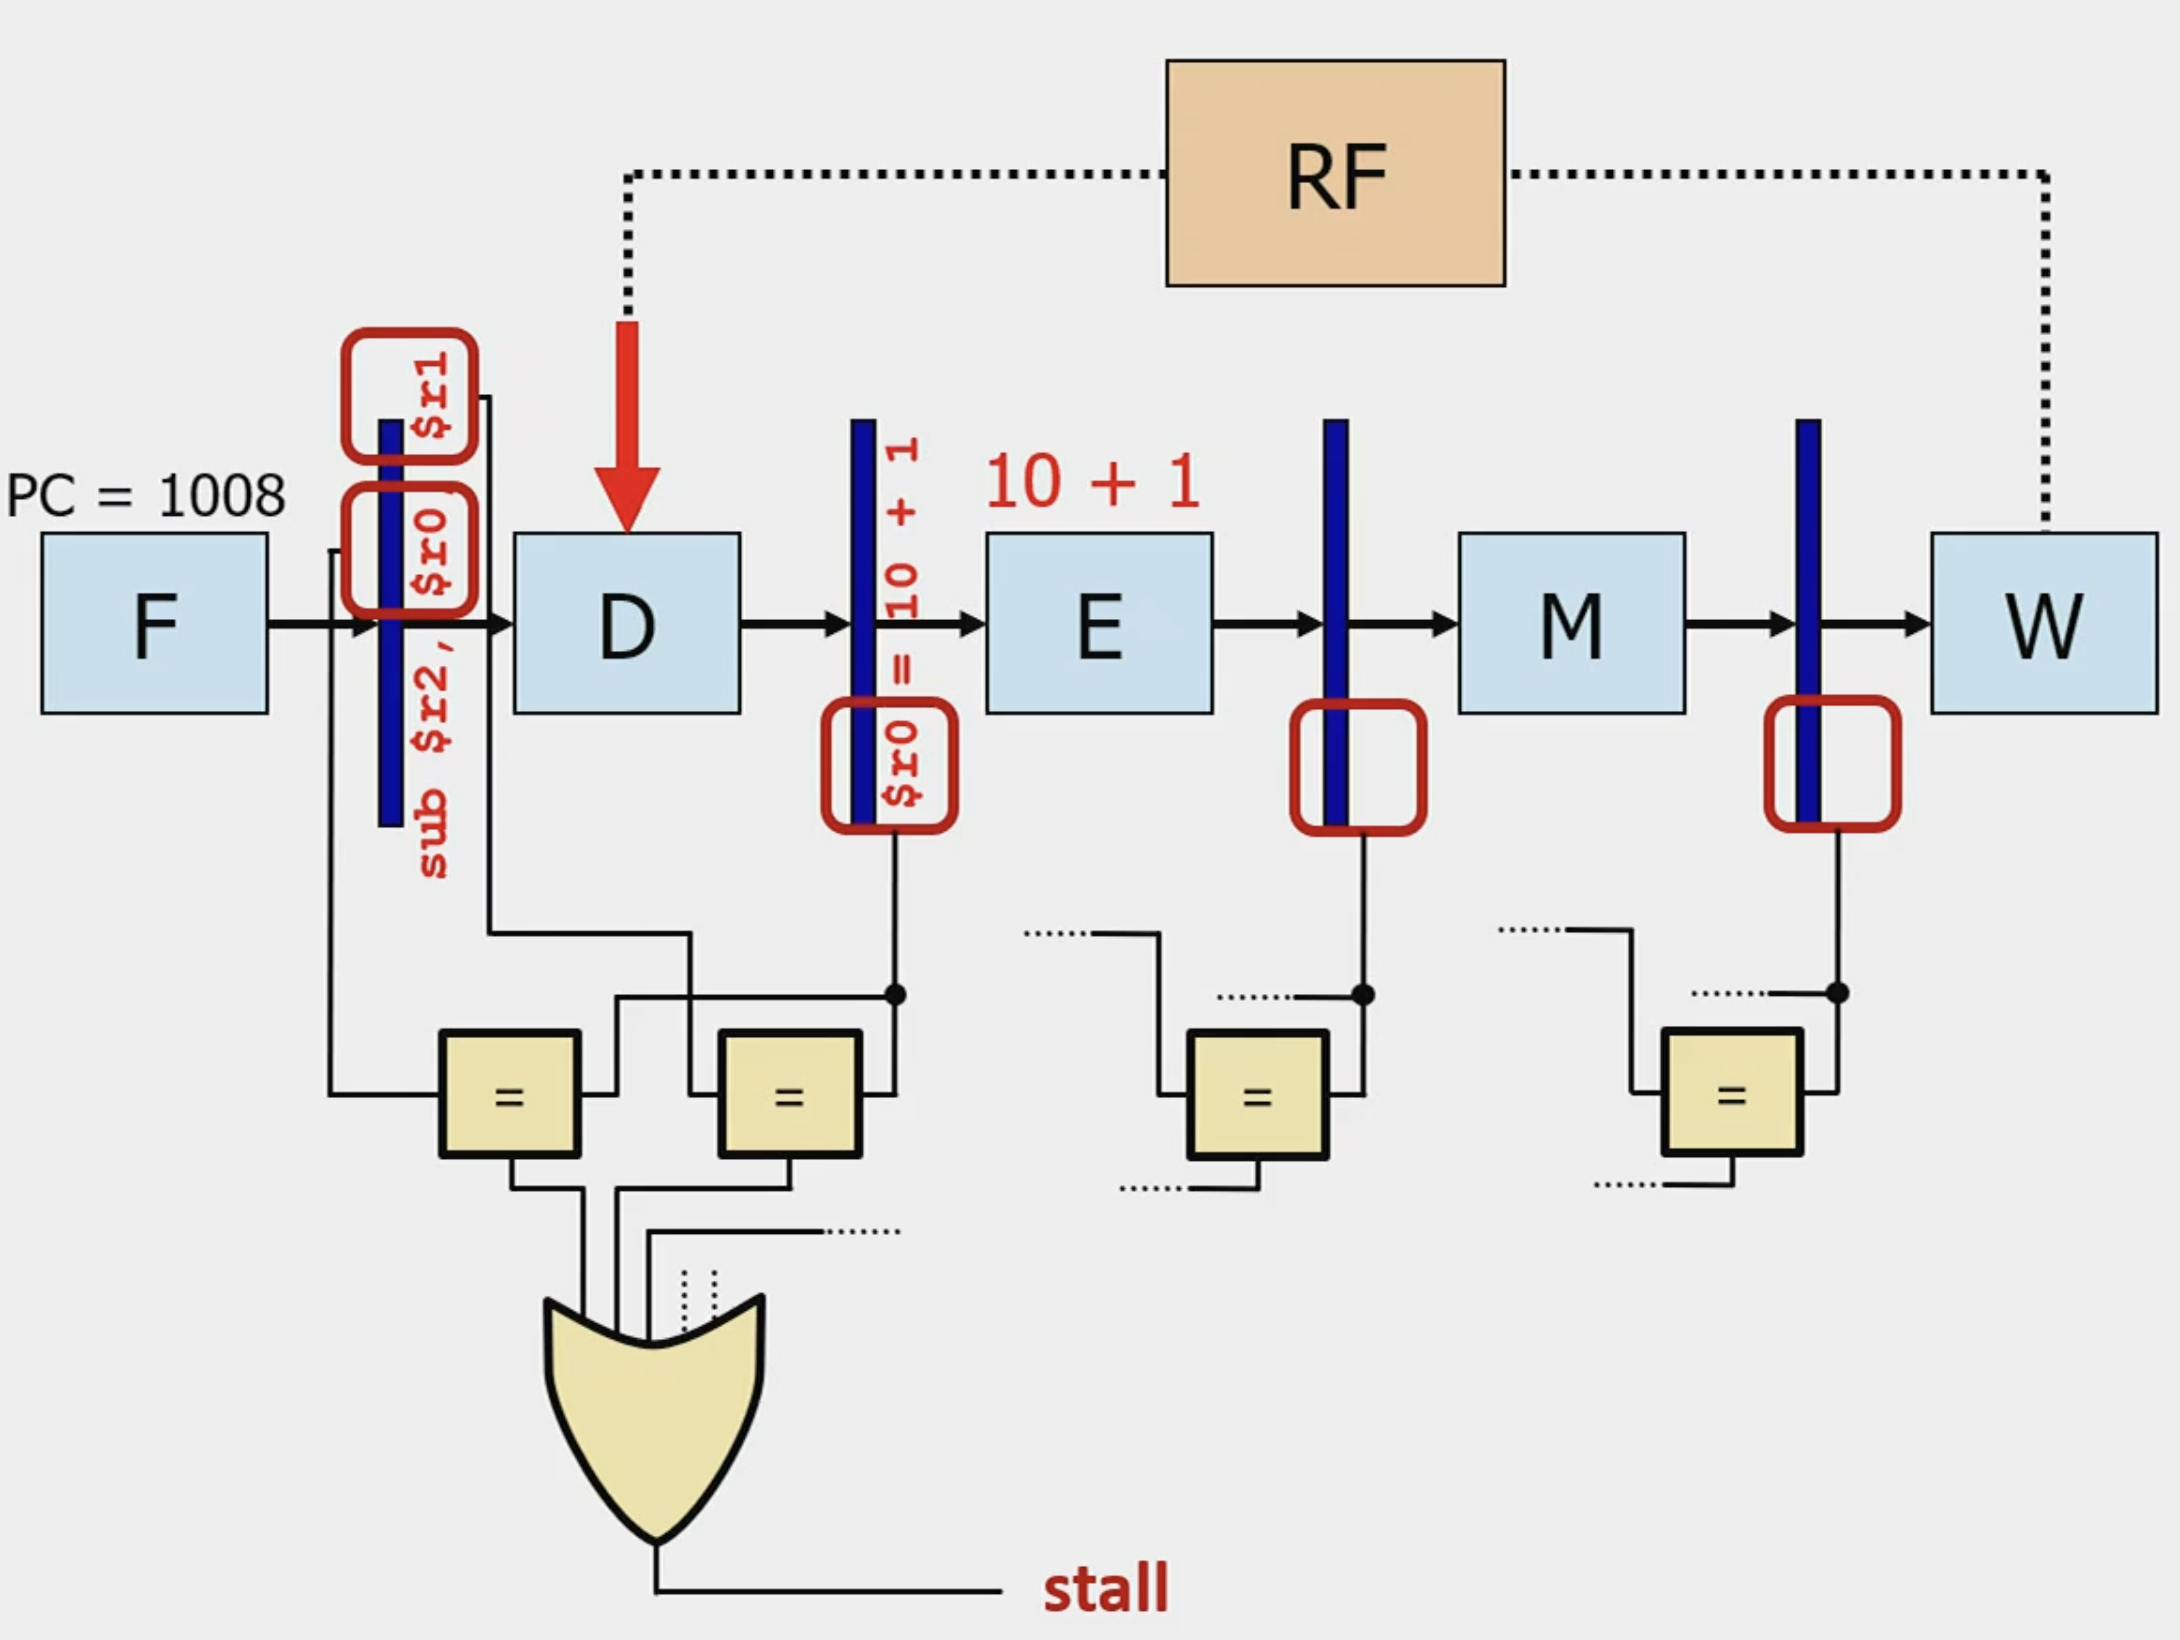
\includegraphics[width=0.45\textwidth]{chapters/chapter4c/images/detect.png}
\end{center}

In this example, a dependency exists between two instructions: the \texttt{sub} instruction in the Decode (D) stage requires the result of the \texttt{addi} instruction, which is still being processed in the Execute (E) stage. The hazard detection unit identifies this dependency and intervenes to maintain correct operation.

\subsection{Stalling in Instruction Execution}
Once a data hazard is detected, the pipeline resolves it using a stalling mechanism. This ensures that dependent instructions do not proceed until the required data becomes available. For the example discussed above, the stalling mechanism operates as follows:
\begin{center}
    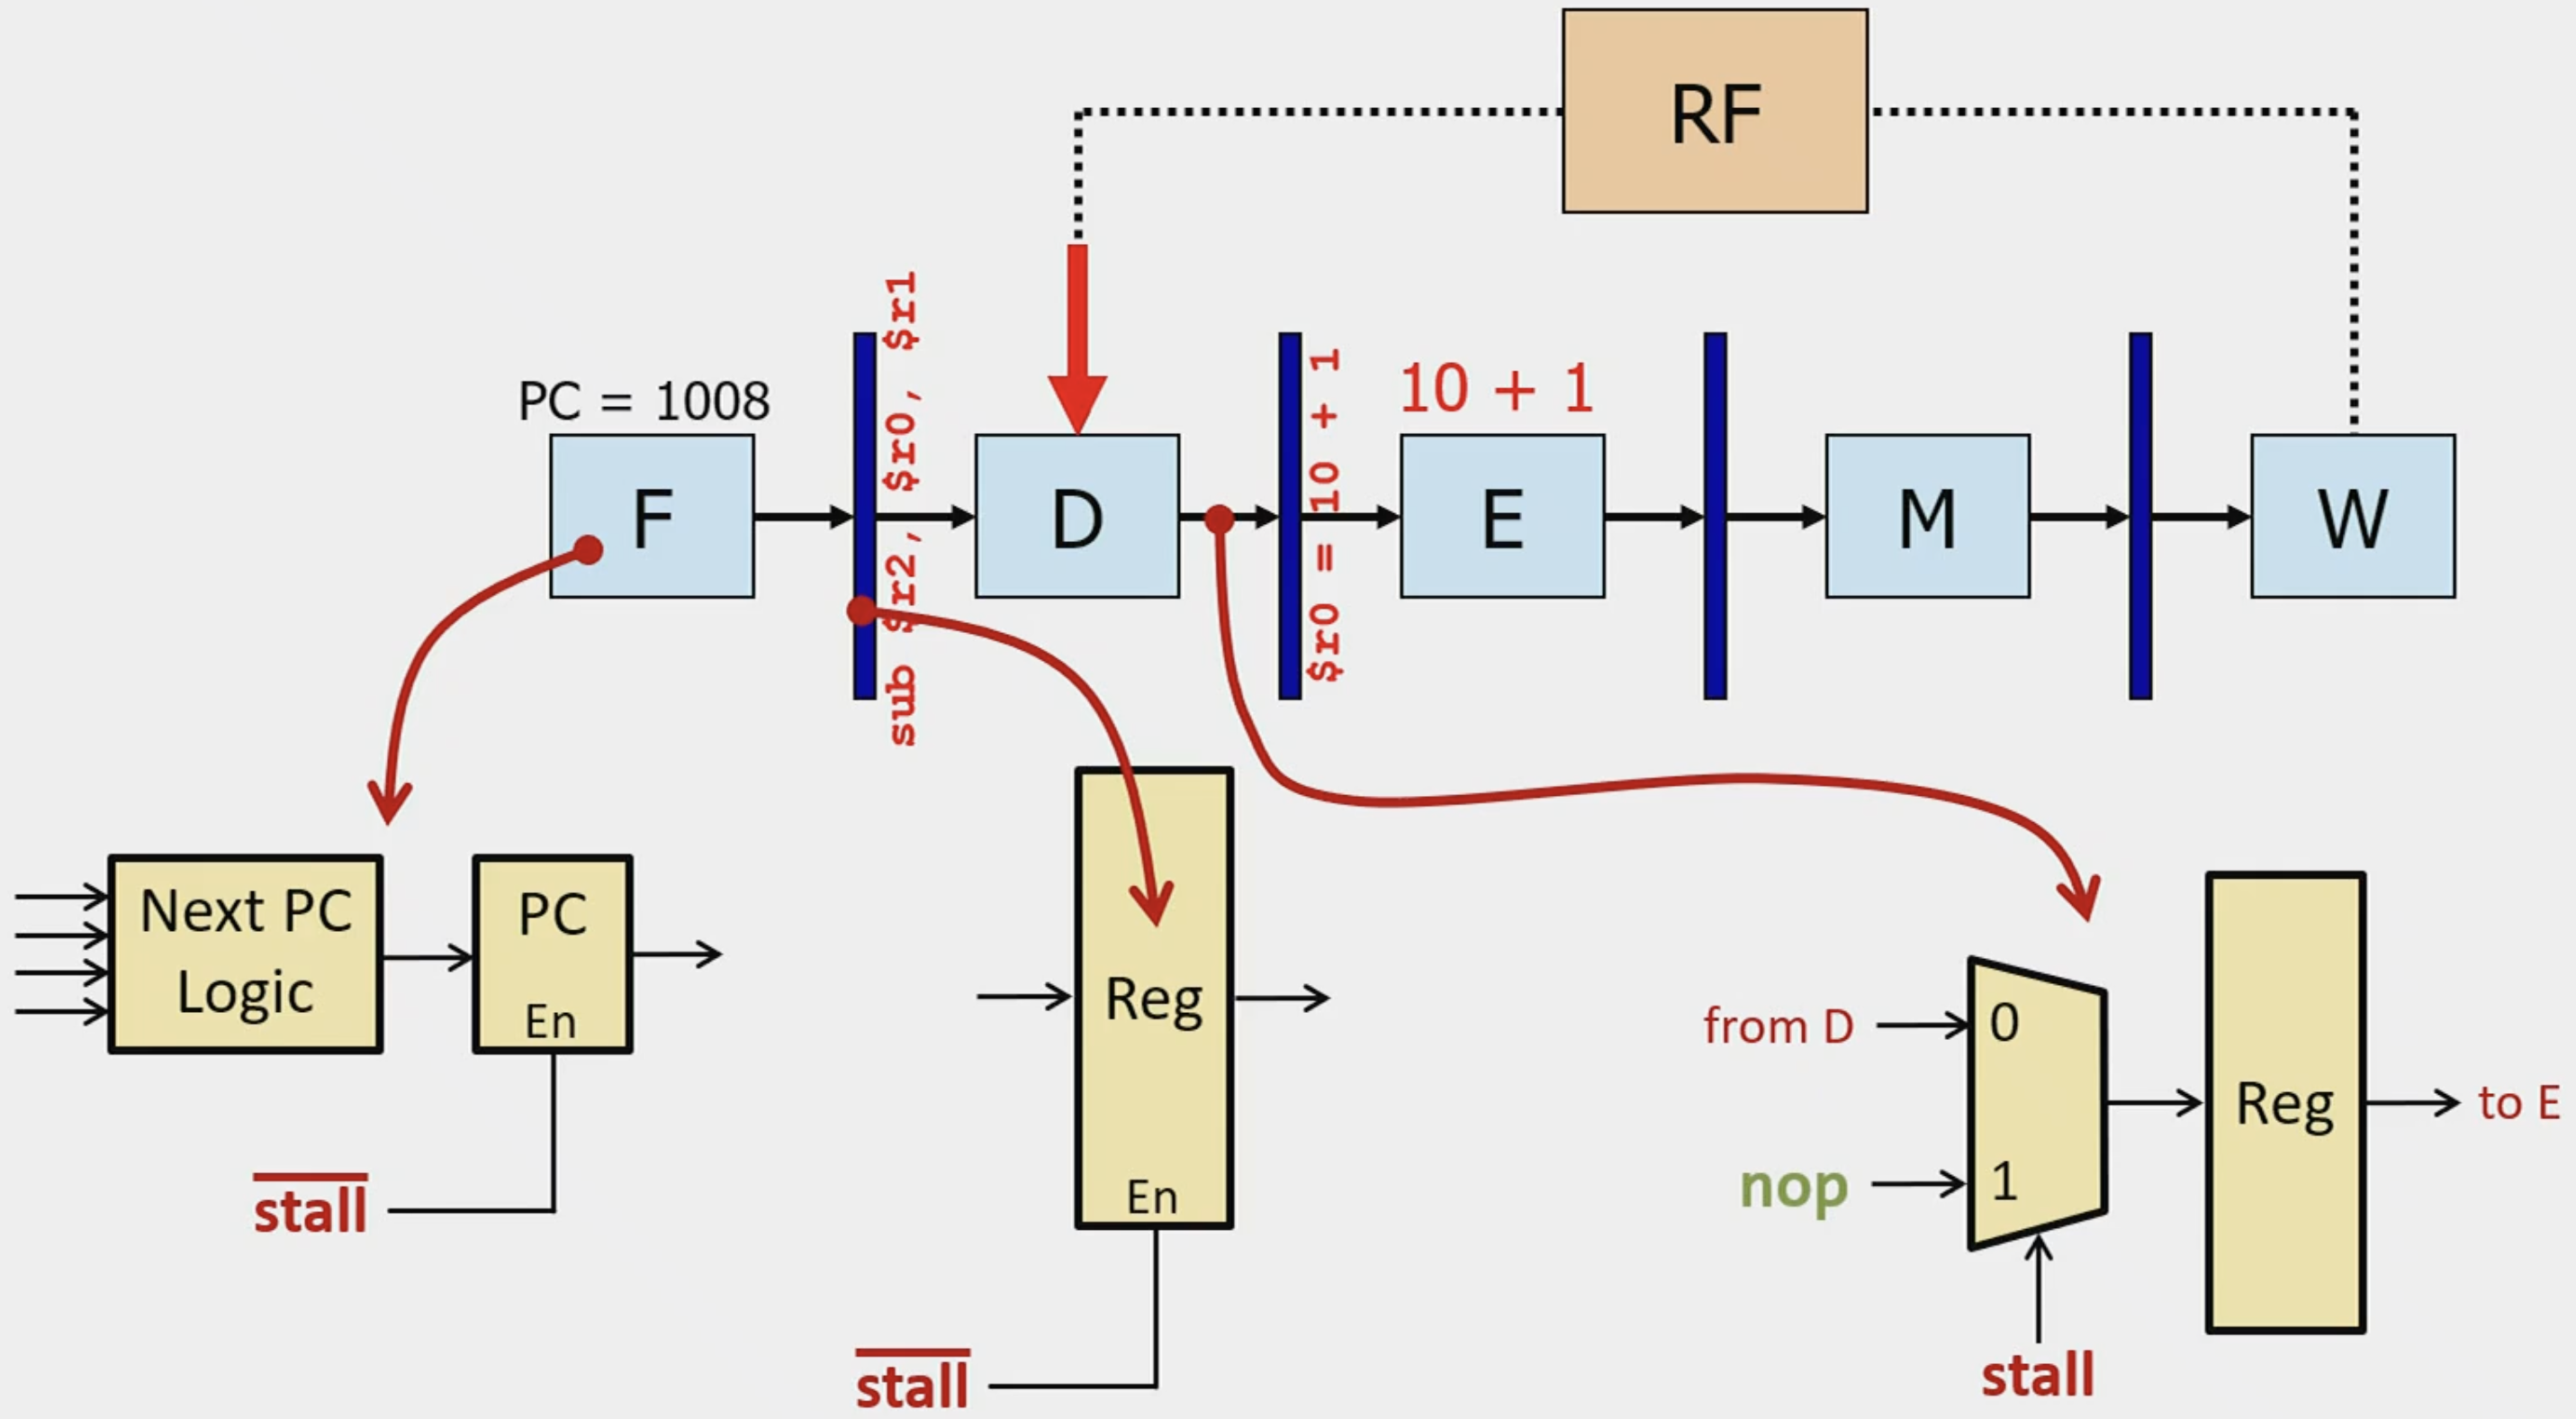
\includegraphics[width=0.65\textwidth]{chapters/chapter4c/images/stalling.png}
\end{center}
\subsubsection*{Stall Mechanism}
When the hazard detection unit identifies a data dependency, it triggers a stall in the pipeline to delay the dependent instruction until the required data becomes available. This is achieved as follows:
\begin{enumerate}
    \item The dependent instruction (e.g., \texttt{sub}) is held in the \textit{Decode (D)} stage until the instruction producing the required data (e.g., \texttt{addi}) computes its result in the \textit{Execute (E)} stage.
    \item A \texttt{nop} (no-operation) instruction is inserted into the pipeline to introduce a delay, allowing the producing instruction to complete its operation.
    \item The control logic halts the Program Counter (PC) and relevant pipeline registers temporarily to synchronize the execution flow.
\end{enumerate}

The flow of execution proceeds as follows:
\begin{itemize}
    \item The producing instruction progresses through the pipeline, computing its result in the \textit{E} stage.
    \item Simultaneously, the pipeline stalls the dependent instruction, holding it in the \textit{D} stage and inserting a \texttt{nop} in the \textit{Execute (E)} stage.
    \item Once the producing instruction writes its result to the register file, the dependent instruction resumes execution using the updated value.
\end{itemize}

While stalling reduces the overall throughput of the pipeline by introducing delays, it is essential for ensuring the correctness of computations. The hazard detection and stalling mechanism together provide a robust solution for managing data dependencies in pipelined processors.

\subsubsection{Conclusion}
By introducing stalling, the updated execution diagram is as follows:
\begin{center}
    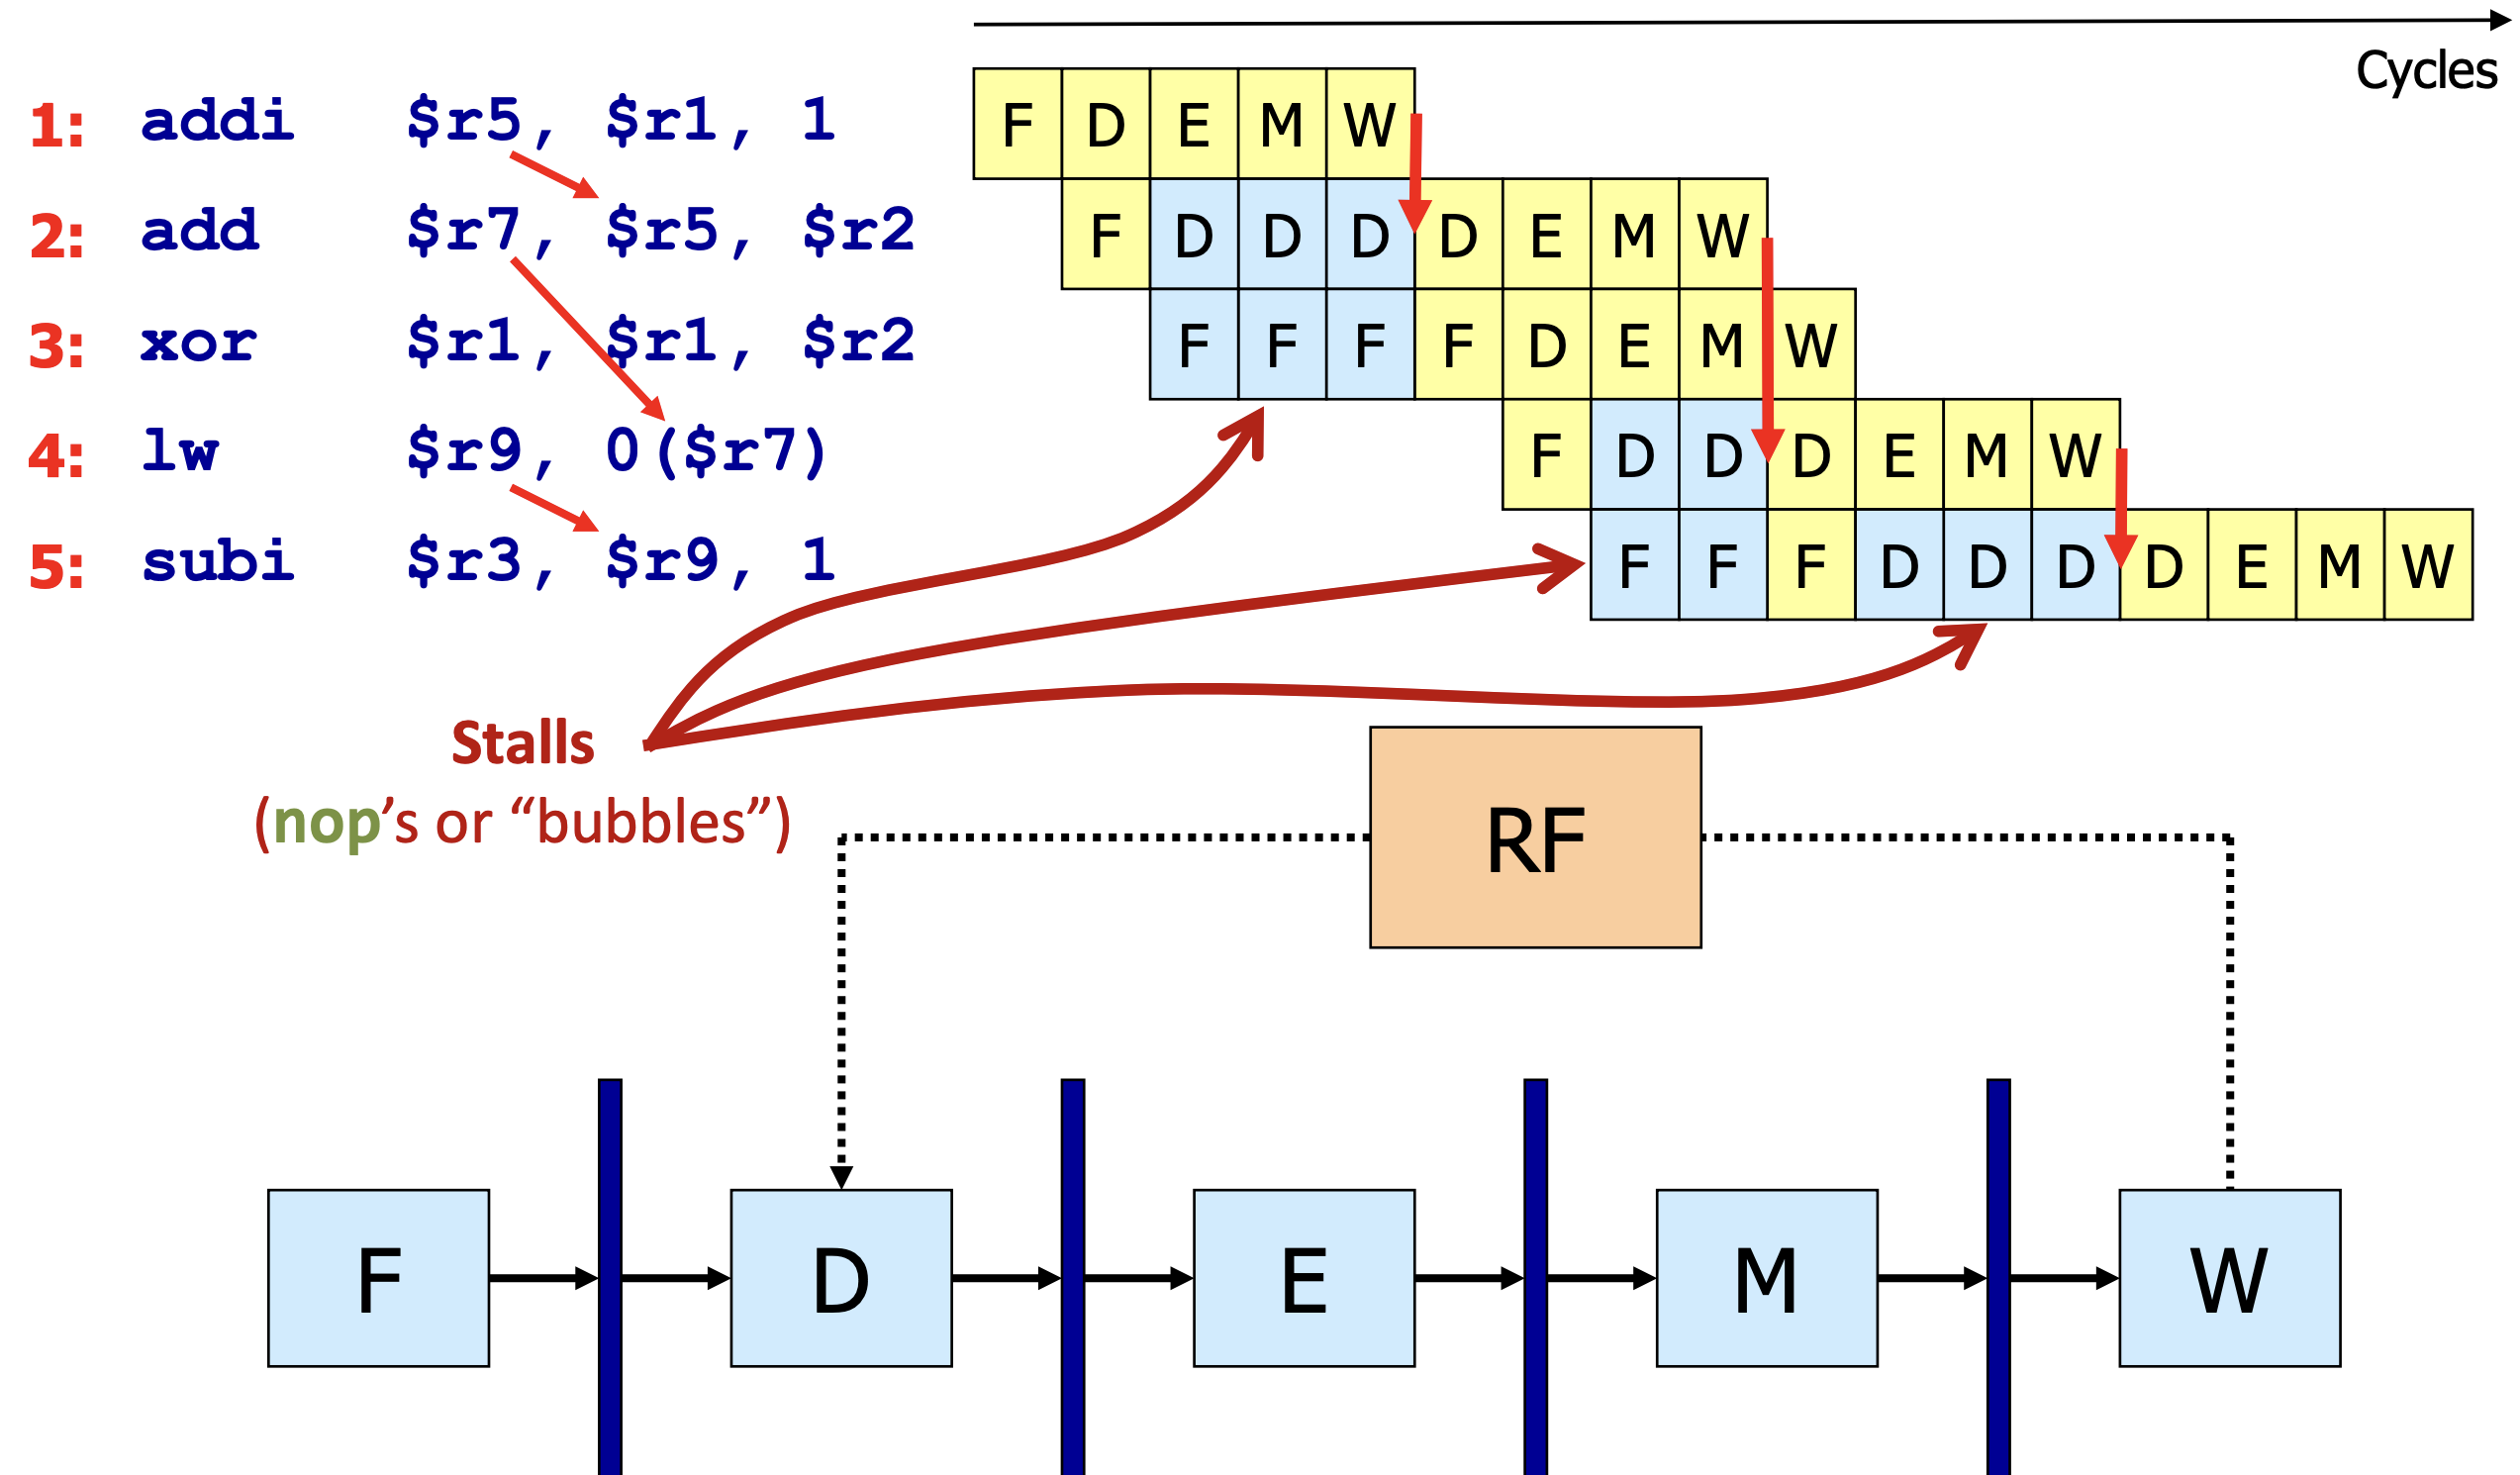
\includegraphics[width=0.65\textwidth]{chapters/chapter4c/images/diag.png}
\end{center}

\subsection{Alternative Solution}
An alternative approach to solving this problem could involve managing stalling in software. For instance, the compiler could statically insert the appropriate number of \texttt{nop} instructions before runtime to avoid any data hazards.
\begin{center}
    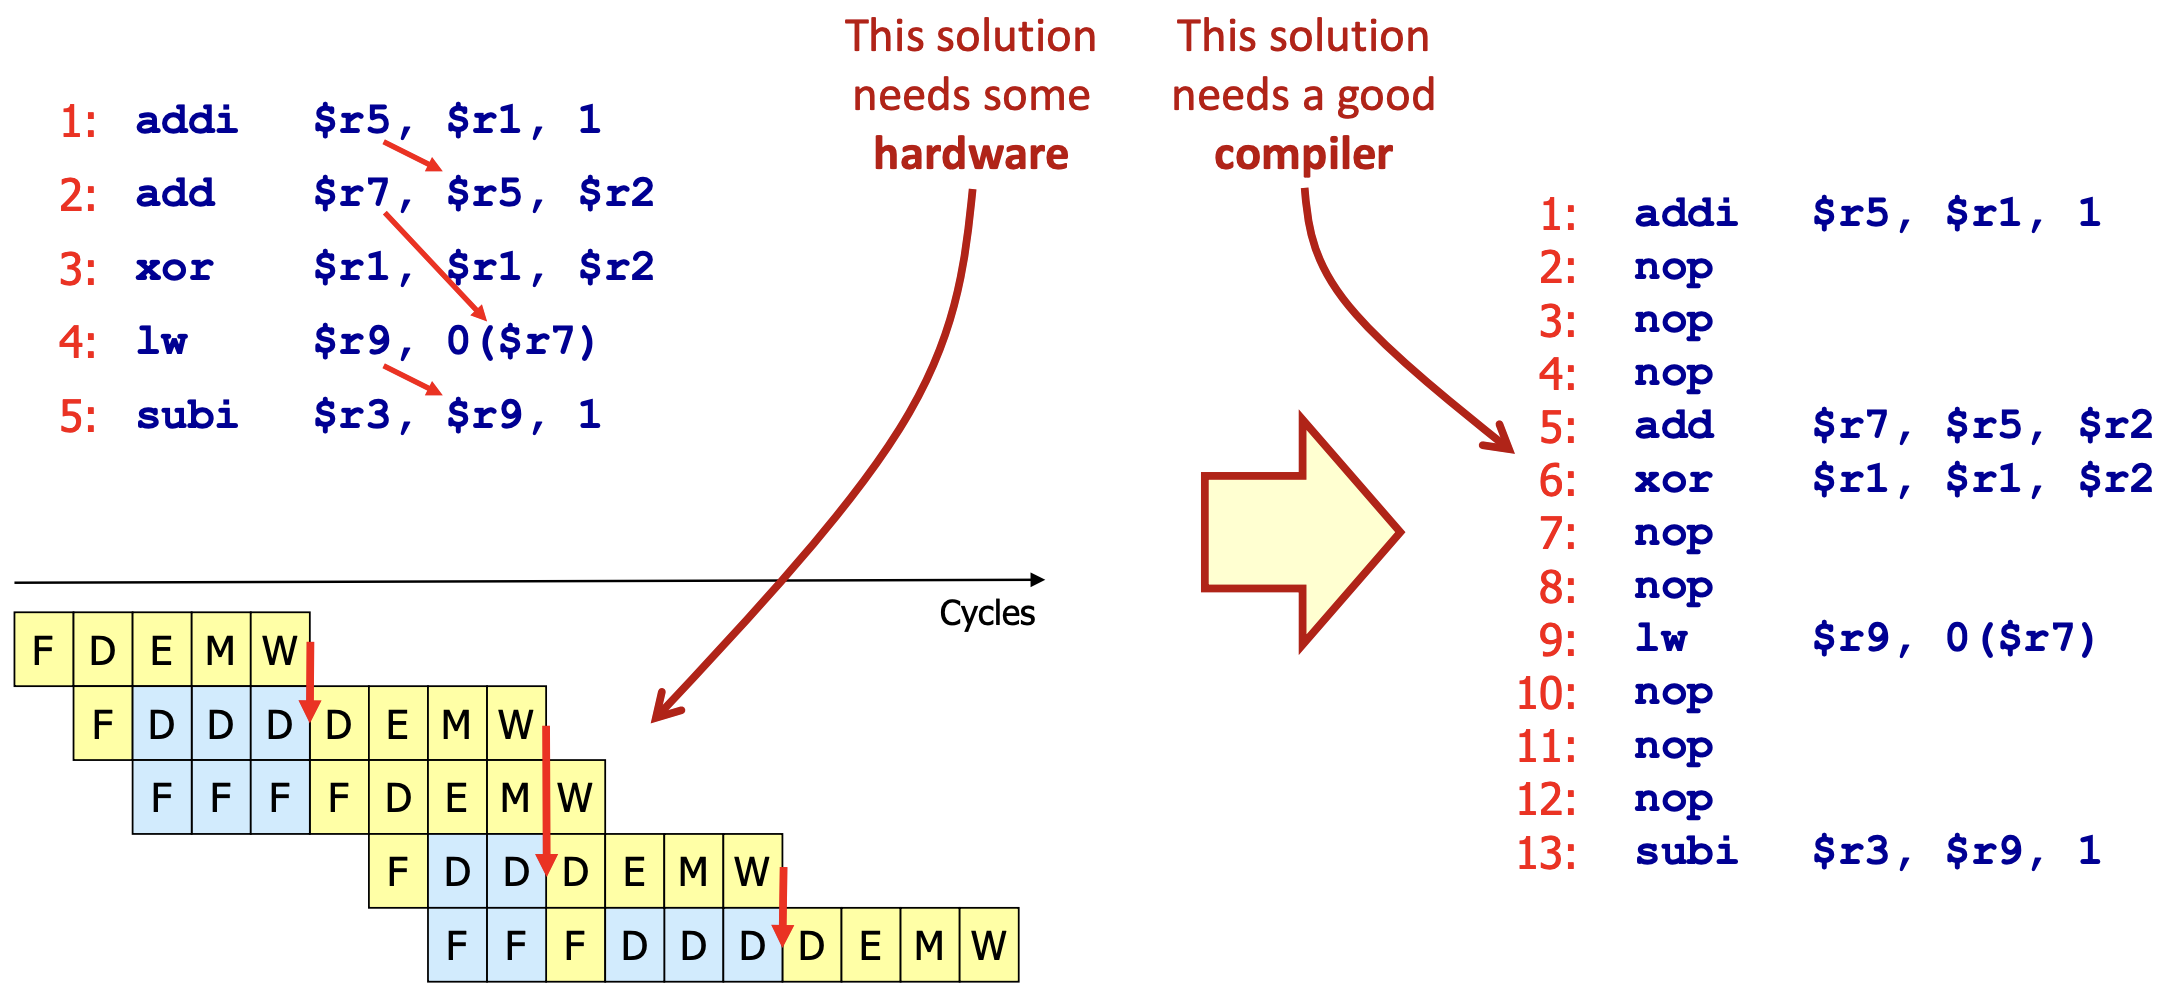
\includegraphics[width=0.65\textwidth]{chapters/chapter4c/images/solution2.png}
\end{center}
\newpage
\subsection{Data Hazards Resolved by Forwarding}
In pipelined processors, data hazards arise when an instruction depends on the result of a previous instruction that has not yet been written to the register file. Forwarding, also known as bypassing, is a hardware technique used to address this issue effectively.
\begin{center}
    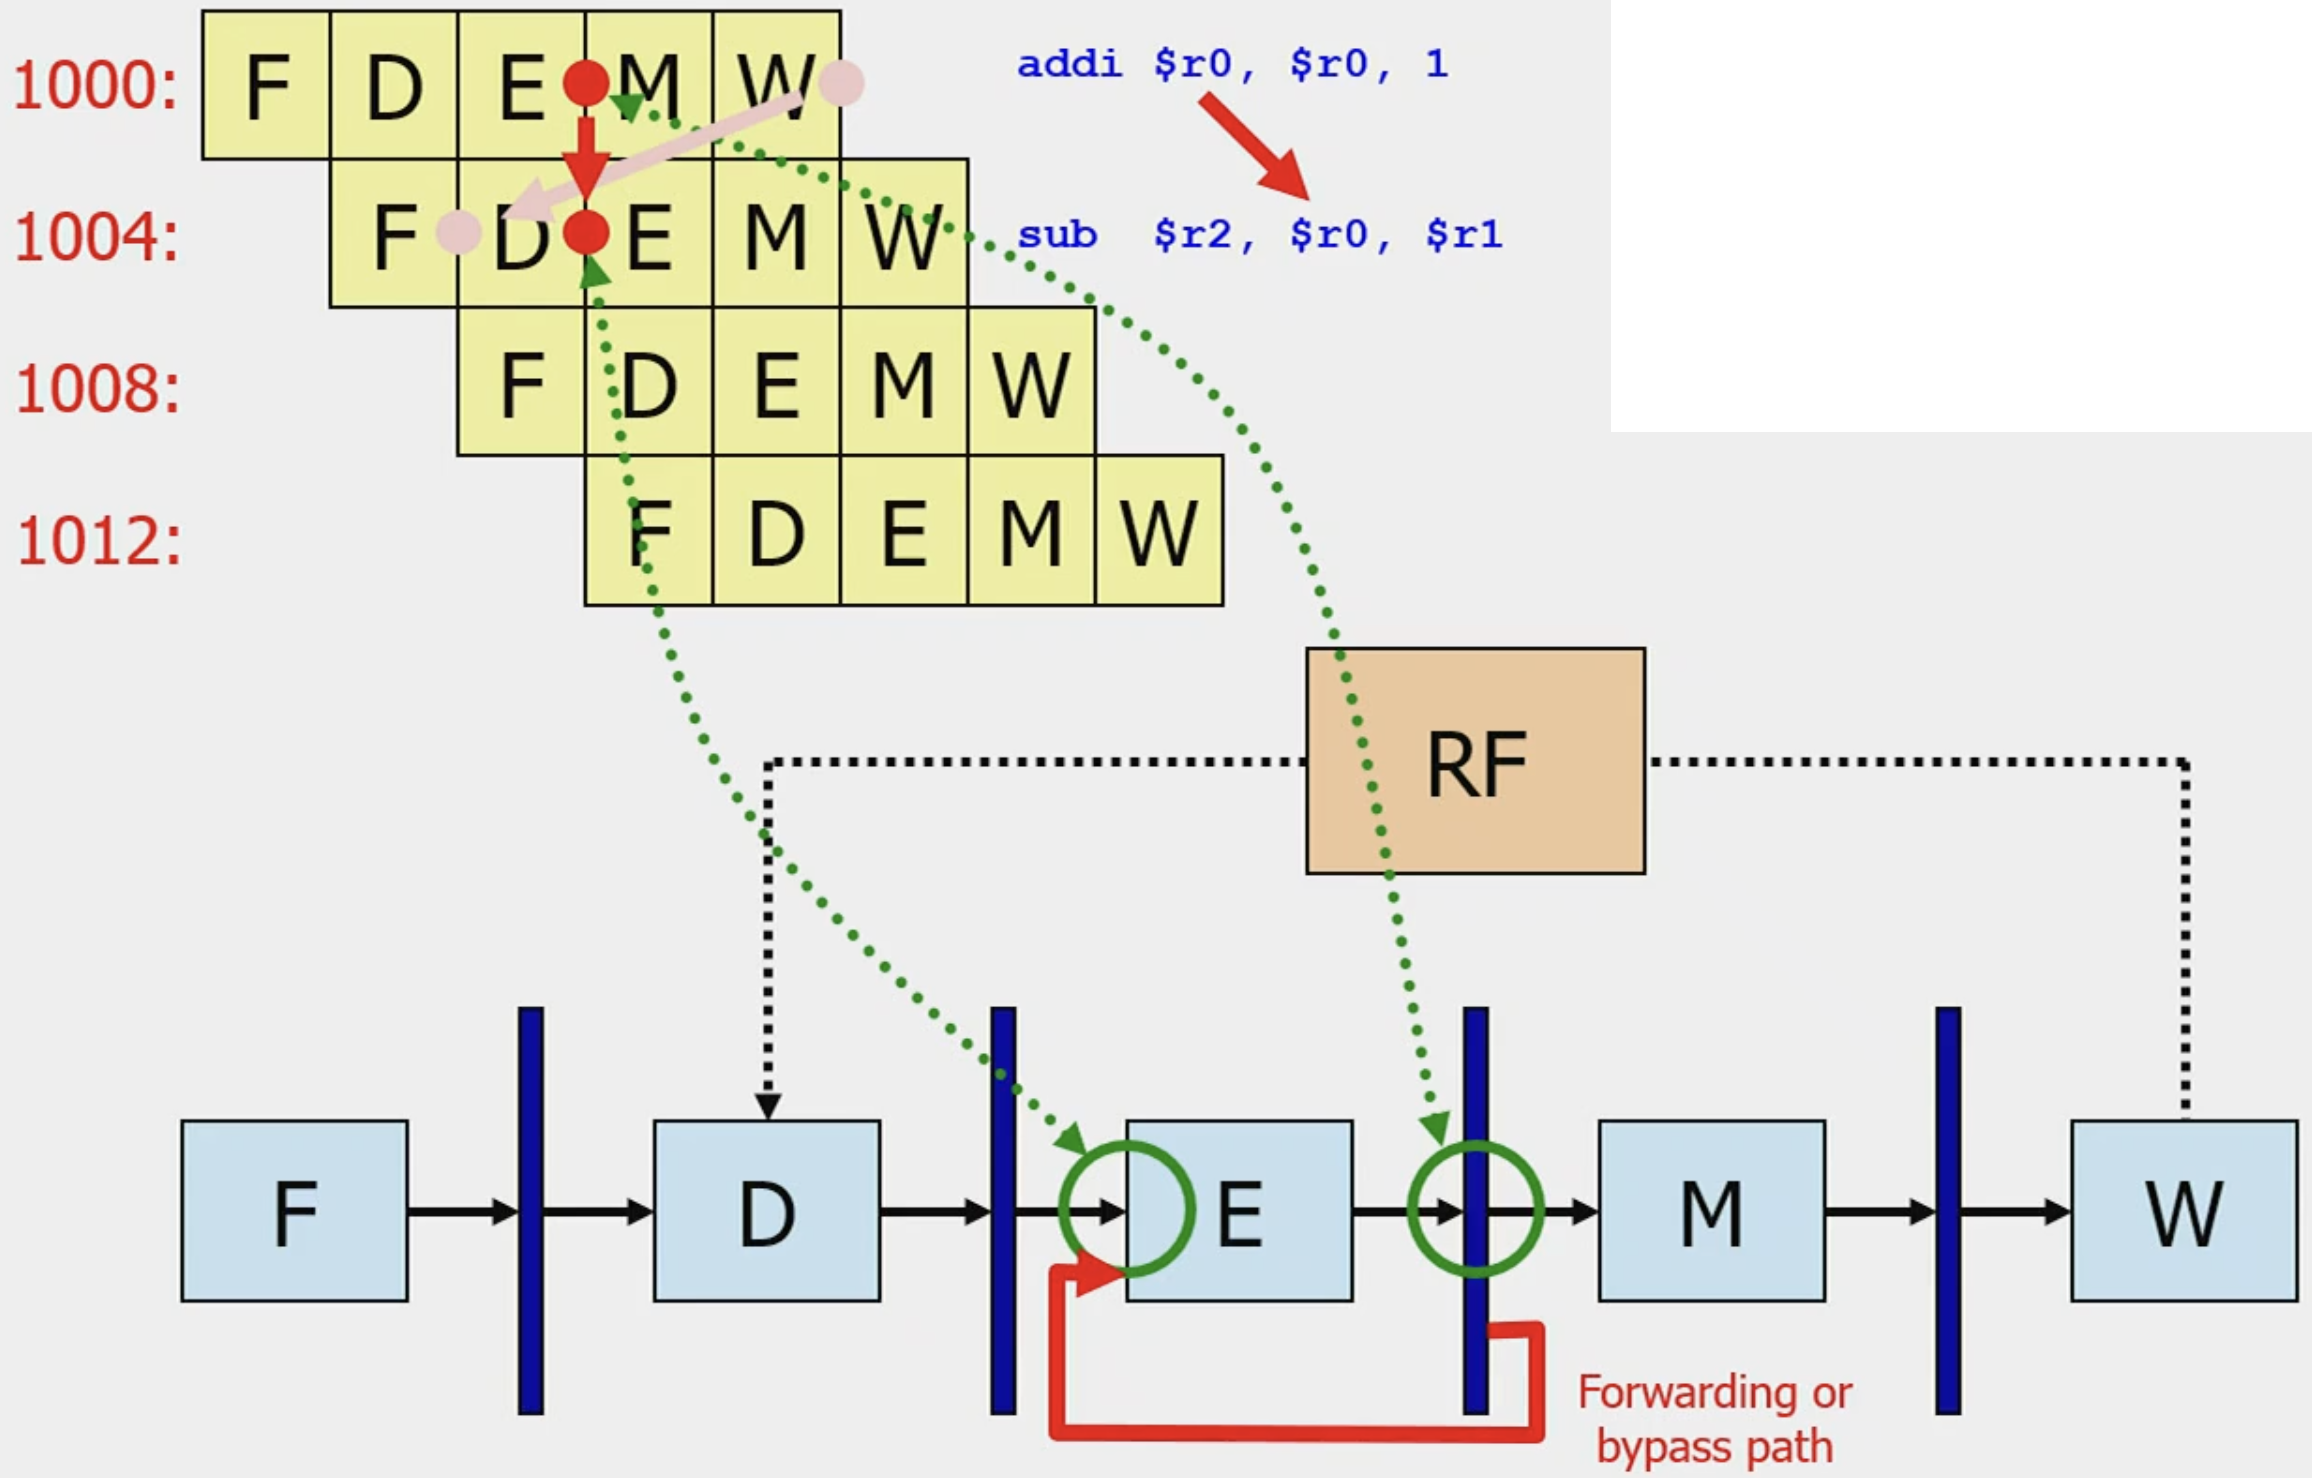
\includegraphics[width=0.65\textwidth]{chapters/chapter4c/images/forwarding.png}
\end{center}
\begin{itemize}
    \item[-] \textbf{Timing vs. Location:} The required data becomes available at the correct time but is not in the necessary location for the dependent instruction.
    \item[-] \textbf{Direct Data Paths:} Forwarding paths are established to transfer data directly from one stage of the pipeline to another, eliminating unnecessary delays.
    \item[-] \textbf{Control Logic:} Additional circuitry, such as multiplexers, is employed to select the appropriate data input during the execute stage.
\end{itemize}

\noindent \textbf{Analogy:} \\
Imagine an assembly line in a factory where one worker produces a component needed by the next worker. Instead of waiting for the component to be placed in storage and then retrieved, the first worker directly hands it to the second worker. Similarly, forwarding allows data to be passed directly between pipeline stages without waiting for it to be written back to the register file.

\noindent \textbf{Example} \\
Consider the following two instructions:
\begin{verbatim}
    addi $r0, $r0, 1
    sub  $r2, $r0, $r1
\end{verbatim}
The result of the \texttt{addi} instruction must be used by the \texttt{sub} instruction. Without forwarding, the pipeline would have to wait until the \texttt{addi} result is written back to the register file before the \texttt{sub} instruction can proceed, causing a stall. With forwarding, the result from the \texttt{addi} instruction is directly sent to the execute stage of the \texttt{sub} instruction, allowing it to proceed without waiting.

\noindent \textbf{Implementation:} \\
The forwarding mechanism introduces hardware paths from:
\begin{itemize}
    \item The \textbf{Execute/Memory} pipeline register back to the Execute stage.
    \item The \textbf{Memory/Write-Back} pipeline register back to the Execute stage.
\end{itemize}
These paths are controlled to ensure that the correct data is provided to the execute stage when needed, bypassing the usual wait for the write-back phase and thereby maintaining the smooth flow of instructions through the pipeline.
\newpage
\subsection{Classic MIPS Pipeline with Forwarding}
\textit{Please take some time to understand this part, }
The classic MIPS pipeline consists of five stages:
\emph{Instruction Fetch}~(\textbf{F}),
\emph{Instruction Decode / Register Read}~(\textbf{D}),
\emph{Execute}~(\textbf{E}),
\emph{Memory Access}~(\textbf{M}),
and
\emph{Write Back}~(\textbf{W}). \\
Forwarding is a mechanism to resolve data hazards by enabling certain results to be directly passed between pipeline stages, bypassing the need for intermediate storage. When fully implemented, forwarding enables the following data paths:

\begin{center}
    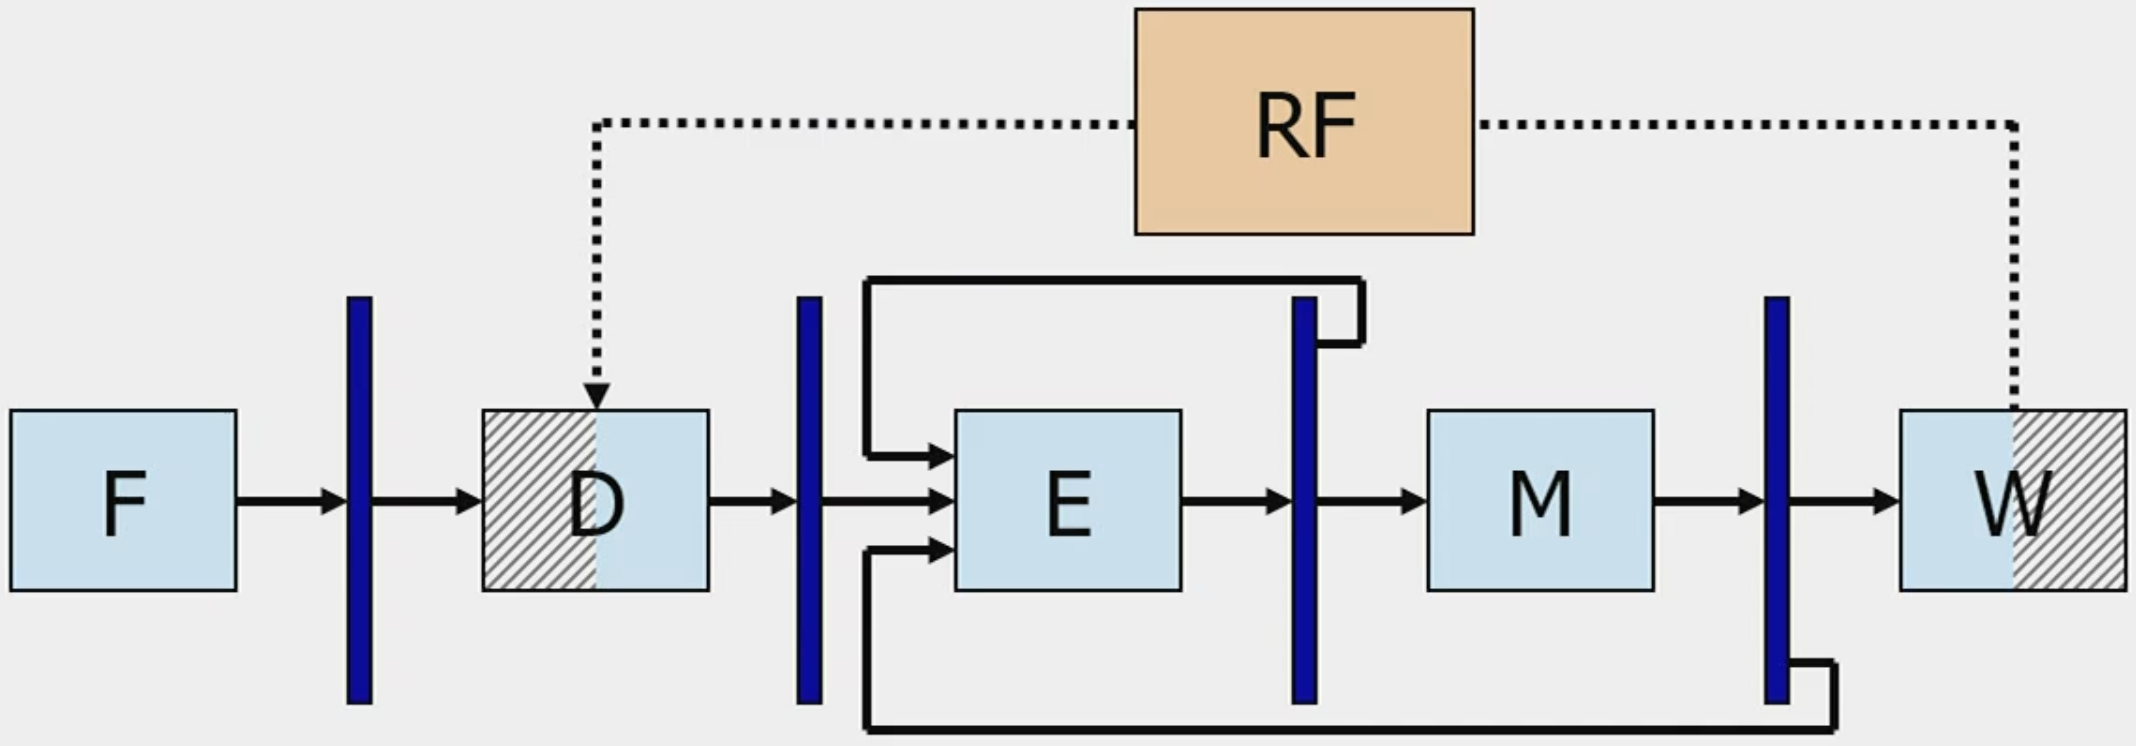
\includegraphics[width=0.45\textwidth]{chapters/chapter4c/images/classic_mips.png}
\end{center}
\begin{itemize}
  \item \textbf{E $\rightarrow$ E:} The output from the Execute stage (\textbf{E}) of one instruction can be forwarded directly to the Execute stage of the next instruction, avoiding dependency-related stalls.
  \item \textbf{M $\rightarrow$ E:} The output from the Memory stage (\textbf{M}) can be forwarded to the Execute stage of the next instruction if required, bypassing the need to wait for the value to reach the Write Back stage.
  \item \textbf{W $\rightarrow$ D:} The output from the Write Back stage (\textbf{W}) can be supplied directly to the Decode stage (\textbf{D}) of a subsequent instruction during the same clock cycle.
\end{itemize}

\noindent
A notable special case is \emph{register-file forwarding} (\textbf{W $\rightarrow$ D}). In this scheme:
\begin{itemize}
  \item During the \textbf{W} stage, registers are written in the \textit{first half} of the clock cycle.
  \item During the \textbf{D} stage, registers are read in the \textit{second half} of the same cycle.
\end{itemize}
\noindent
This timing ensures that a register value written in \textbf{W} is immediately available for reading in \textbf{D}, avoiding a read-after-write hazard for consecutive instructions.

\noindent
In the classic MIPS pipeline, the forwarding paths described (\textbf{E $\rightarrow$ E}, \textbf{M $\rightarrow$ E}, \textbf{W $\rightarrow$ D}) are sufficient to resolve most data hazards. However, some instruction sequences may still require additional stall cycles if the needed forwarding path is unavailable.
\newpage
\section{Structural Hazards}

A \textbf{structural hazard} occurs when multiple instructions simultaneously require the same hardware resource (e.g., pipeline stage or memory port), potentially causing pipeline stalls or incorrect execution.

\begin{center}
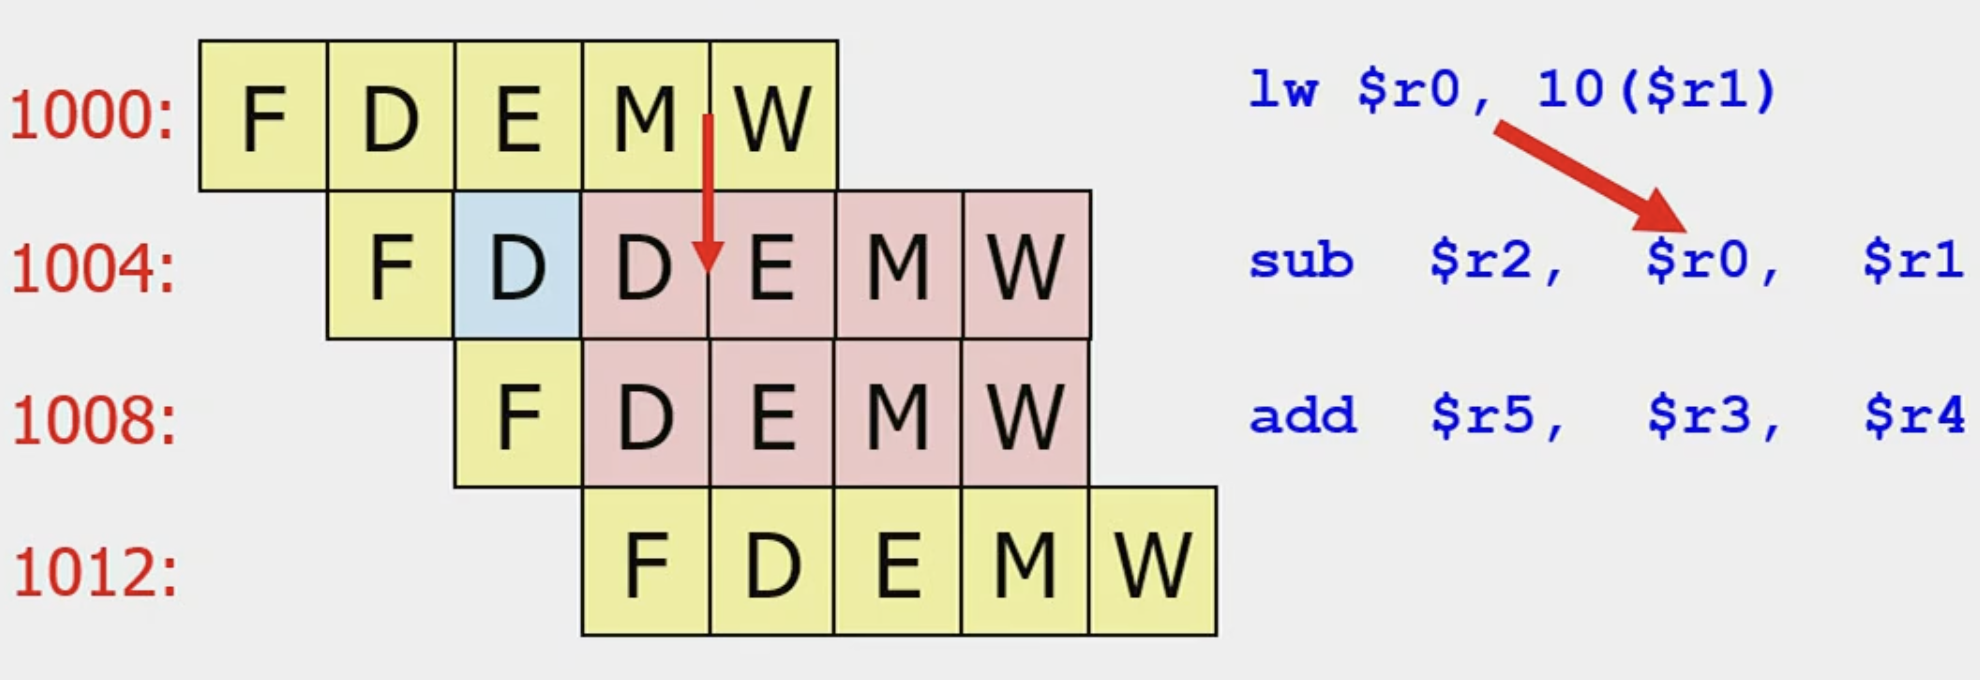
\includegraphics[width=0.45\textwidth]{chapters/chapter4c/images/struct_hazard.png}
\end{center}

\subsubsection{Example}

Consider the following instruction sequence:

\begin{verbatim}
1. lw   $r0, 0($r1)      # Load word into $r0
2. lw   $r2, 4($r1)      # Load word into $r2
3. add  $r3, $r0, $r2    # Add $r0 and $r2, store in $r3
\end{verbatim}

In a pipelined processor with a single memory port, both \texttt{lw} instructions (1 and 2) attempt to access memory during the Memory (M) stage simultaneously. This conflict creates a structural hazard, forcing the processor to stall one instruction until the memory resource becomes available, thereby reducing throughput.

\subsubsection{Handling Cache Misses}

Cache misses can introduce structural hazards by stalling pipeline stages:

\begin{itemize}
    \item A miss in the Memory (M) stage can block access to memory or the bus, causing stalls in the Execute (E), Decode (D), and Fetch (F) stages.
\end{itemize}

\subsubsection{Stalling Strategies}

\begin{itemize}
    \item \textbf{Single Cache Miss}:
        \begin{itemize}
            \item Stall the Memory (M) stage and all preceding stages (E, D, F).
            \item Allow the Write-Back (W) stage to proceed to avoid blocking completed operations.
        \end{itemize}
    \item \textbf{Concurrent Misses}:
        \begin{itemize}
            \item Prioritize data cache misses over instruction cache misses to minimize overall stall time.
            \item This may temporarily cause resource contention on main memory.
        \end{itemize}
\end{itemize}

\subsubsection{Consequences of Unresolved Structural Hazards}

\begin{itemize}
    \item Instructions may execute out of order or prematurely, leading to resource conflicts.
    \item This can result in incorrect execution or pipeline corruption.
\end{itemize}

\subsubsection{Prevention in Our Pipeline}

\begin{itemize}
    \item Careful resource allocation ensures that structural hazards are \textbf{avoided}.
    \item Adequate provisioning of each pipeline stage and proper management of shared resources enable concurrent operation without contention.
\end{itemize}

\subsubsection{Dependency Example}

In the example above, the \texttt{sub} instruction depends on the result of the \texttt{lw} instruction (\$r0). If \$r0 is not ready when \texttt{sub} reaches the Execute stage, a structural hazard can occur unless stalls or forwarding mechanisms are implemented to handle the dependency.
\newpage
\section{Control Hazards in Pipelined Processors}

\subsection{The Problem}
A \emph{control hazard} (or \emph{branch hazard}) occurs in a pipelined CPU whenever the next instruction to fetch depends on the result of a branch. Since pipeline stages operate in parallel, the processor often fetches an instruction \emph{before} it knows whether the branch will be taken or not. If the branch is taken, the speculatively fetched instruction is wrong and must be \emph{flushed} (or invalidated); if the branch is not taken, execution continues normally.

\begin{center}
\textbf{Pipeline Stages:} F (Fetch), D (Decode), E (Execute), M (Memory), W (Write-back)
\end{center}

\subsubsection{Example}
\begin{verbatim}
Address   Instruction
----------------------------------
1000      beq   $r0, $r1, loop
1004      sub   $r2, $r0, $r1
1008      ...   (next instruction)
\end{verbatim}

When the CPU starts to fetch the instruction at \texttt{1004}, it may not yet know if the branch at \texttt{1000} is taken. If the branch is taken, the fetched instruction at \texttt{1004} is incorrect and must be discarded.

\subsection{Stalling (Flushing) the Pipeline}
One straightforward solution is to \emph{stall} the pipeline until it is known whether the branch will be taken. Conceptually:
\begin{enumerate}
  \item Fetch the branch instruction.
  \item Stall new instruction fetches until the branch outcome is computed (e.g., by the end of the E stage).
  \item If the branch is taken, jump to the correct target address; if not, continue with the sequential address.
\end{enumerate}
Stalling ensures correctness, but it \textbf{wastes several cycles} whenever a branch is encountered.

\begin{itemize}
  \item \textbf{Fetching \& Decoding a wrong instruction} is not harmful as long as it is not \emph{executed}.
  \item If the branch resolves in the E stage (cycle 3 for a 5-stage pipeline), two extra instructions may have been fetched speculatively. If the branch is taken, those two instructions are \emph{killed} (flushed); if not, they continue without delay.
\end{itemize}

\subsection{Delay Slots}
Another approach, historically used by MIPS and a few others, is to define \emph{delay slots} after a branch. In a 1-slot design:
\begin{enumerate}
  \item The instruction \emph{immediately} following the branch is always executed (the ``delay slot'').
  \item The branch effect (taken or not taken) occurs \emph{after} that delay slot instruction completes.
\end{enumerate}
Hence, the architecture enforces that instructions in the delay slot \emph{always} run, regardless of whether the branch is taken. In a 2-slot design, the next two instructions always execute, and so on.

\begin{center}
\textbf{Example of inserting NOPs (no-ops) in delay slots:}
\end{center}
\begin{verbatim}
1:   beq  $r0, $r1, loop  <-- branch
2:   nop                  <-- delay slot #1
3:   nop                  <-- delay slot #2
4:   sub $r2, $r0, $r1    <-- next real instruction
\end{verbatim}
While legal, using NOPs in delay slots merely shifts the stall problem into software. More sophisticated compilers attempt to move independent instructions into these slots so that the extra cycles are not wasted.


\section{Summary}

Pipelining in computer architecture can be hindered by three primary types of hazards:

\begin{itemize}
    \item \textbf{Data Hazards} (\textit{data dependences}): These occur when instructions depend on the results of previous instructions.
    \begin{itemize}
        \item \textit{Solutions:}
        \begin{itemize}
            \item Forwarding paths, wherever possible.
            \item Stalls, in all other cases.
        \end{itemize}
    \end{itemize}

    \item \textbf{Control Hazards} (\textit{jumps and branches}): These arise from the control flow of instructions, such as branches and jumps.
    \begin{itemize}
        \item \textit{Solutions:}
        \begin{itemize}
            \item Delay slots, if the architecture allows it.
            \item Branch prediction, to try to do the right thing.
            \item Stalls, if the above are not feasible.
        \end{itemize}
    \end{itemize}

    \item \textbf{Structural Hazards} (\textit{conflicting need for a resource}): These occur when multiple instructions require the same hardware resource simultaneously.
    \begin{itemize}
        \item \textit{Solutions:}
        \begin{itemize}
            \item Design rigid pipelines that avoid structural hazards by construction.
            \item Use stalls in cases where hazards cannot be avoided.
        \end{itemize}
    \end{itemize}
\end{itemize}
